\begin{tikzpicture}
  \definecolor{gray}{HTML}{9b9b9b}
  \node[anchor=south west,inner sep=0] (image) at (0,0) {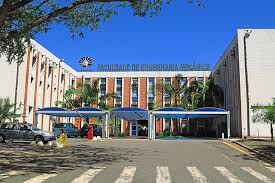
\includegraphics[width=0.75\textwidth]{./photos/fem.jpg}};
  \begin{scope}[x={(image.south east)},y={(image.north west)}]
    % \node [anchor=east] (lfe) at (1.05, 0.5) {LFE};
    \node [anchor=east, white] (fcv-101) at (0.65, 0.93) {FCV-101};
    \node [anchor=east, white] (pt-101) at (0.65, 0.85) {PT-101};
    \node [anchor=east, white] (pdt-101) at (0.65, 0.65) {PDT-101};
    \node [anchor=east, white] (tt-101) at (0.83, 0.45) {TT-101};
    
    \node [anchor=east, white, fill=black, inner sep=1pt, opacity=0.1, text opacity=1] (lfe) at (0.83, 0.58) {Laminar flow element};
    \node [anchor=west, white] (nozz) at (0.5,0.38) {Injector Nozzle};
    % \draw[red,ultra thick,rounded corners] (0.48,0.80) rectangle (0.55,0.95);

    \draw[-latex, line width=4pt, white] (fcv-101) to[out=0, in=180] (0.78,0.93);
    \draw[-latex, line width=4pt, white] (pt-101) to[out=0, in=90] (0.87,0.78);
    \draw[-latex, line width=4pt, white] (pdt-101) to[out=0, in=-90] (0.8,0.76);
    \draw[-latex, line width=4pt, white] (tt-101) to[out=0, in=235] (0.93,0.52);

    \draw[-latex, line width=4pt, white] (lfe) to[out=0, in=180] (0.9,0.58);
    \draw[-latex, line width=4pt, white] (nozz) to[out=180, in=45] (0.215,0.245);
  \end{scope}
\end{tikzpicture}%
